\documentclass[12pt, titlepage]{article}

\usepackage{fullpage}
\usepackage[round]{natbib}
\usepackage{multirow}
\usepackage{booktabs}
\usepackage{tabularx}
\usepackage{graphicx}
\usepackage{float}
\usepackage{xr}
\usepackage{xr-hyper}
\usepackage{hyperref}
\hypersetup{
    colorlinks,
    citecolor=blue,
    filecolor=black,
    linkcolor=red,
    urlcolor=blue
}

\usepackage{longtable}
\usepackage[utf8]{inputenc}
\usepackage{amsmath, mathtools}
\usepackage{amsfonts}
\usepackage{amssymb}
\usepackage{colortbl}
\usepackage{hyperref}
\usepackage{longtable}
\usepackage{xfrac}
\usepackage{siunitx}
\usepackage{caption}
\usepackage{pdflscape}
\usepackage{fixltx2e}
\usepackage{afterpage}
\usepackage{seqsplit}
\usepackage{underscore}
\usepackage{lscape}
\usepackage[english]{babel}
\usepackage[T1]{fontenc}
\usepackage{nameref}
%\usepackage{enumitem}

\makeatletter
\let\orgdescriptionlabel\descriptionlabel
\renewcommand*{\descriptionlabel}[1]{%
  \let\orglabel\label
  \let\label\@gobble
  \phantomsection
  \edef\@currentlabel{#1}%
  %\edef\@currentlabelname{#1}%
  \let\label\orglabel
  \orgdescriptionlabel{#1}%
}
\makeatother

%% Comments

\usepackage{color}

\newif\ifcomments\commentstrue %displays comments
%\newif\ifcomments\commentsfalse %so that comments do not display

\ifcomments
\newcommand{\authornote}[3]{\textcolor{#1}{[#3 ---#2]}}
\newcommand{\todo}[1]{\textcolor{red}{[TODO: #1]}}
\else
\newcommand{\authornote}[3]{}
\newcommand{\todo}[1]{}
\fi

\newcommand{\wss}[1]{\authornote{blue}{SS}{#1}} 
\newcommand{\plt}[1]{\authornote{magenta}{TPLT}{#1}} %For explanation of the template
\newcommand{\an}[1]{\authornote{cyan}{Author}{#1}}

%% Common Parts

\newcommand{\progname}{Mechatronics Engineering} % PUT YOUR PROGRAM NAME HERE
\newcommand{\authname}{Team \# 34, ParkingLotHawk
\\ Fady Zekry Hanna, zekryhf
\\ Winnie Trandinh, trandint
\\ Muhammad Ali, alim102
\\ Muhammad Khan, khanm120} % AUTHOR NAMES                  

\usepackage{hyperref}
    \hypersetup{colorlinks=true, linkcolor=blue, citecolor=blue, filecolor=blue,
                urlcolor=blue, unicode=false}
    \urlstyle{same}
                                

\externaldocument{../../HazardAnalysis/HazardAnalysis}
\externaldocument{../../SRS/SRS}

\setcounter{secnumdepth}{4}
\setcounter{tocdepth}{4}

%\newcounter{acnum}
%\newcommand{AC\arabic{acnum}}{AC\theacnum}
%\newcommand{AC\arabic{acnum}}{AC\arabic{acnum}}
%\newcommand{AC\ref}[1]{AC\ref{#1}}

%\newcounter{ucnum}
%\newcommand{UC\arabic{ucnum}}{UC\theucnum}
%\newcommand{\uref}[1]{UC\ref{#1}}

%\newcounter{mnum}
%\newcommand{\mthemnum}{M\themnum}
%\newcommand{\mref}[1]{M\ref{#1}}

\begin{document}

\title{Module Guide for \progname{}} 
\author{\authname}
\date{\today}

\maketitle

\pagenumbering{roman}

\section{Revision History}

\begin{tabularx}{\textwidth}{p{3cm}p{2cm}X}
\toprule {\bf Date} & {\bf Version} & {\bf Notes}\\
\midrule
January 18, 2023 & 1.0 & Initial Revision\\
\bottomrule
\end{tabularx}

\newpage

\section{Reference Material}

There are no external references used within this document.

\subsection{Abbreviations and Acronyms}

\renewcommand{\arraystretch}{1.2}
\begin{tabular}{p{3cm} p{12cm}} 
  \toprule		
  \textbf{symbol} & \textbf{description}\\
  \midrule 
  AC & Anticipated Change\\
  DAG & Directed Acyclic Graph \\
  M & Module \\
  MG & Module Guide \\
  MIS & Module Interface Specifications \\
  OS & Operating System \\
  R & Requirement\\
  Algo & Algorithms \\
  SRS & Software Requirements Specification\\
  \progname & Mechatronics Engineering is an engineering stream that mixes electrical, mechanical, and software engineering.\\
  UC & Unlikely Change \\
  DDC & Drone Decision and Control \\
  Ardupilot & Open-source Autopilot Software Suite for unmanned vehicles. \\
  ROS Node & Process using ROS functionality. \\
  MavROS & Process presents a ROS interface to interact with Ardupilot and MAVLINK. \\
  High-level Motion Commands & 3-dimensional move to commands, e.g. hover at 5m, move 5m left, etc. \\
  MAVLINK & Typical communication network used by hardware peripherals, low-level interface. \\
  ROS & Robot Operating System, open-source robotics middleware suite. \\
  main & Starting point of execution for a process. \\
  PC & Personal Computer. \\
  \bottomrule
\end{tabular}\\

\newpage

\tableofcontents

\listoftables

\listoffigures

\newpage

\pagenumbering{arabic}

\section{Introduction}

The practice of breaking down a system into smaller, manageable parts, called modules, is a common method used in software development. Each module is assigned to a programmer or programming team as a task. We suggest using a method of decomposition that follows the principle of information hiding. This approach allows for flexibility in future changes as the "hidden information" within each module represents potential changes. This is particularly useful in scientific computing, where modifications and adjustments are often made during the early stages of development as the problem is being explored.  

Our design follows the principles of information hiding. Information hiding is a concept in computer science and software engineering that refers to the technique of hiding internal information and state of a software module from other modules to reduce the dependencies between them. The rules we follow are as follows:

\begin{itemize}
\item System details that are likely to change independently should be the secrets of separate modules.
\item Each data structure is implemented in only one module.
\item Any other program that requires information stored in a module’s data structures must obtain it by calling access programs belonging to that module.
\end{itemize}

The Module Guide (MG) is developed after the first stage of design, the Software Requirements Specification (SRS) is completed. The MG outlines the modular structure of the system and serves as a guide for both designers and maintainers to easily identify the different parts of the software. This document can be used by several groups of readers: new project members can use it as a guide to quickly understand the overall structure and find the relevant modules they need, maintainers can use it to improve their understanding of the system when making changes and update the relevant sections after changes have been made, and designers can use it to check for consistency, feasibility, and flexibility in the design, such as consistency among modules, the feasibility of the decomposition, and flexibility of the design.

The remaining portion of the document is organized as follows: Section \ref{SecChange} lists the expected and unexpected changes to the software requirements. Section \ref{SecMH} provides a summary of how the system was divided into modules based on the likely changes. Section \ref{SecConnection} outlines the connections between the software requirements and each individual module. Section \ref{SecMD} offers a detailed explanation of each module. Section \ref{SecTM} includes two traceability matrices, one to confirm that the design meets the requirements outlined in the SRS and another that shows the relationship between anticipated changes and the modules. Finally, Section \ref{SecUse} explains the relationship between different modules.
\section{Anticipated and Unlikely Changes} \label{SecChange}

This section lists possible changes to the system. According to the likeliness
of the change, the possible changes are classified into two
categories. Anticipated changes are listed in Section \ref{SecAchange}, and
unlikely changes are listed in Section \ref{SecUchange}.

\subsection{Anticipated Changes} \label{SecAchange}

Anticipated changes are the source of the information that is to be hidden
inside the modules. Ideally, changing one of the anticipated changes will only
require changing the one module that hides the associated decision. The approach
adapted here is called design for
change.

\begin{description}
\item[AC1 \label{AC_Ardupilot1}:] Interfacing with sensors to read data and share it on the MAVLINK Network.

\item[AC2 \label{AC_Ardupilot2}:] Interfacing with actuators to read and follow commands on the MAVLINK Network. 

\item[AC3 \label{AC_Ardupilot3}:] 
Control algorithms that make the drone follow high level motion commands. 

\item[AC4 \label{AC_MavROS1}:] 
Presentation of all sensor and firmware status information into ROS Topics.  

\item[AC5 \label{AC_MavROS2}:] 
Presentation of the API to control the drone in the form of ROS Services and ROS Topics.  

\item[AC6 \label{AC_BaseSocket1}:] 
Rudimentary LAN Socket used by higher level modules for LAN communication. There are various types of different sockets, and multiple standards regarding the interface they implement.

\item[AC7 \label{AC_MessageSocket1}:] 
High-level communication interface used to send and receive string data between Drone and Operator. 

\item[AC8 \label{AC_GStreamer1}:] 
Framework used for creating video streams to send video from the drone to the Operator's PC. 

\item[AC9 \label{AC_DroneCamera1}:] 
Interfacing with camera hardware to get the latest live image.

\item[AC10 \label{AC_DroneCamera2}:] 
Framework for the creation of the video streaming pipeline, and routines to send images over it. Components of the pipeline may include compression, communication, and decompression.

\item[AC11 \label{AC_OperatorCamera1}:] 
Receiving images from the video stream created by the drone and presenting them in a simple-to-use API for modules running on the Operator's PC. 

\item[AC12 \label{AC_UserInterface1}:] 
Choice and layout of interface widgets, e.g. buttons, dropdown boxes, maps, images, etc.

 \item[AC13 \label{AC_UserInterface2}:] 
Display of parking lot information to the Operator (occupancy map, live video stream). 

 \item[AC14 \label{AC_UserInterface3}:] 
Display of drone information, e.g. current location, current altitude, health status, etc.

 \item[AC15 \label{AC_MainInterfaceModule1}:] 
The starting point of execution (main function) for the process running the Operator's PC. 

 \item[AC16 \label{AC_ROS1}:] 
Message passing system used for inter-process communication on the drone. 

 \item[AC17 \label{AC_AlgorithmTopicInterface1}:] 
Subscription and extraction of data from ROS Topics to read   data needed by the various Algorithm's e.g. if an algorithm module needs a different sensor reading then one module should be modified to provide the sensor reading.

 \item[AC18 \label{AC_AlgorithmTopicInterface2}:] 
The ROS Topic Publisher's needed by Algorithm's process to publish their results to other processes.

 \item[AC19 \label{AC_DDCTopicInterface1}:] 
Subscription and extraction of data from ROS Topics to read   data needed by the various Operations processes e.g. if an Operation State specified in the SRS needs a different sensor reading then one module should be modified to provide the sensor reading.
 
 \item[AC20 \label{AC_DDCTopicInterface2}:] 
The ROS Topic Publisher's needed by Operation's modules to command/instruct the drone.

 \item[AC21 \label{AC_DDCServiceInterface1}:] 
Calling of ROS Services by the Operations modules, as well as processing the responses returned from the services i.e. there are a plethora of ROS Services that do different things and that have different conventions with respect to calling them.

 \item[AC22 \label{AC_VisionApp1}:] 
Visual perception algorithm used to yield insights from the raw parking lot images.

 \item[AC23 \label{AC_MappingApp1}:] 
Environment mapping algorithm used to create an occupancy map of the parking lot.

\item[AC24 \label{AC_PathPlanApp1}:] 
Choosing the next location for the drone to move to.

\item[AC25 \label{AC_PathPlanApp2}:] 
Path planning algorithm that suggests the optimal path for further exploration of the parking lot.

\item[AC26 \label{AC_AlgorithmManagerApp1}:] 
Routines for managing the execution and data exchange between the sub-algorithms.

\item[AC27 \label{AC_MainAlgorithmModule1}:]
The starting point of execution (main function) for the process running the algorithm modules. 

\item[AC28 \label{AC_OperationState1}:]
Routines that implement the state machine specified in the SRS, i.e. the states and transitions in the SRS may change. 

\item[AC29 \label{AC_OperationManager1}:]
Presentation of data/information for the operation state routines to make decisions. 

\item[AC30 \label{AC_OperationManager2}:]
Presentation of services needed by the operation state routines to command/instruct the drone, e.g. a new operation state may require a different type of command/instruction to implement its required behavior.
 
\item[AC31 \label{AC_OperationManager3}:]
Management of operation state, i.e. storing the current operation state and calling its routines appropriately.

\item[AC32 \label{AC_MainDDCModule1}:]
The starting point of execution (main function) for the process running the operations. 

\end{description}


\subsection{Unlikely Changes} \label{SecUchange}

\begin{description}
\item[UC1 \label{UC_1}:] 	Flight controller hardware its associated sensors: The decision to use a flight controller was quite straight forward, as it saves a lot of development time. It offers a multitude of hardware interfacing and control algorithm services, meaning the team will not have to develop such low-level moduls. It makes the project much more feasible. Flight controller is an expensive purchase, thus once this decision is made it becomes even more expensive to change the hardware.
\item[UC2 \label{UC_2}:] 		Firmware (Ardupilot): Although there are other firmware options with the chosen flight controller, Ardupilot comes associated with the purchased flight controller. This is also the most popular and dominant firmware used in most drone projects.

\item[UC3 \label{UC_3}:] 		Edge Compute device: The Raspbery PI is the officially supported compute device for the chosen Flight Controller.  

\item[UC4 \label{UC_4}:] 
Edge Compute Power: The drone's frame and size limitations make adding another compute device unfeasible. Thus the drone's  compute power is limited to that of a Raspberry Pi PI.

\item[UC5 \label{UC_5}:] 
Canadian Laws regarding Drones: Laws regarding the drone's maximum frame size limit the choices of frame size and mechanical design.

\item[UC6 \label{UC_6}:] 
Operating System (OS) of the User Interface: The OS was specified to be Windows in the SRS. Windows is also the most common OS used in a professional setting.
\item 
\end{description}

\section{Module Hierarchy} \label{SecMH}

This section provides an overview of the module design. Modules are summarized
in a hierarchy decomposed by secrets in Table \ref{TblMH}. The modules listed
below, which are leaves in the hierarchy tree, are the modules that will
actually be implemented.

\subsection{Launched Modules}
Among the many modules, there are five modules that are run as standalone processes. Modules run on the drone's hardware include \nameref{Main DDC Module}, \nameref{Main Algorithm Module}, \nameref{MavROS}, and \nameref{ROS} (also known as the master node). On the Operator's PC, the \nameref{Main Interface Module} is run.


\begin{table}[h!]
\centering
\begin{tabular}{p{0.3\textwidth} p{0.4\textwidth}  p{0.3\textwidth}}
\toprule
\textbf{Level 1} & \textbf{Level 2} & 
\textbf{Level 3}\\
\midrule
{Hardware Hiding} & 
Ardupilot \\
& MavROS \\
\midrule
Communication Hiding &
Drone-PC Communication Hiding & Base Socket \\
 && Message Socket \\
 && GStreamer \\
 && Drone Camera \\
 && Operator Camera \\
 &{Drone Inter-Process Communication Hiding} 
& ROS \\
&& Algorithm Topic Interface \\
&& DDC Topic Interface \\
&& DDC Service Interface \\
\midrule
Interface Hiding
& User Interface \\
& Main Interface Module \\
\midrule
{Algorithm Hiding} 
& Vision App \\
& Mapping App \\
& Path Planning App \\
& Algorithm Manager App \\
& Main Algorithm Module \\
\midrule
{Drone Decision and Control (DDC) Hiding} 
& Operation States \\
& Operations Manager \\
& Main DDC Module \\
\midrule
\end{tabular}
\caption{Module Hierarchy}
\label{TblMH}
\end{table}

\section{Connection Between Requirements and Design} \label{SecConnection}

The design of the system is intended to satisfy the requirements developed in
the SRS. In this stage, the system is decomposed into modules. The connection
between requirements and modules is listed in Table~\ref{TblRT}.

\section{Module Decomposition} \label{SecMD}

Modules are decomposed according to the principle of ``information hiding''
proposed by \citet{ParnasEtAl1984}. The \emph{Secrets} field in a module
decomposition is a brief statement of the design decision hidden by the
module. The \emph{Services} field specifies \emph{what} the module will do
without documenting \emph{how} to do it. For each module, a suggestion for the
implementing software is given under the \emph{Implemented By} title. If the
entry is \emph{OS}, this means that the module is provided by the operating
system or by standard programming language libraries.  \emph{\progname{}} means the
module will be implemented by the \progname{} software.

Only the leaf modules in the hierarchy have to be implemented. If a dash
(\emph{--}) is shown, this means that the module is not a leaf and will not have
to be implemented.

\subsection{Hardware Hiding Modules \label{Hardware Hiding Modules}}

\begin{description}
\item[Secrets:] The secret of this module is the interfacing with hardware in a manner to present the software modules with an easy to use interface for reading sensor data, processing sensor data, and sending motion commands.
\item[Services:] Presents sensor data as ROS Topics. Presents a high-level motion command interface through ROS Topics and ROS Services.
\item[Implemented By:] -

\subsubsection{Firmware Module}
\label{Firmware}
\begin{description}
\item[Secrets:]The secret of this module is interfacing the drone's hardware with the MAVLINK Interface.
\item[Services:] Shares sensor data with the MAVLINK interface. Makes the drone follow high-level motion commands given by the MAVLINK interface, by utilizing control algorithms to instruct the actuator hardware. Examples of high-level commands include hovering at a given height, moving to a certain location, landing at a location, etc.
\item[Implemented By:] Ardupilot, an open source unmanned vehicle Autopilot Software Suite, capable of controlling autonomous
\item[Type of Module:] Library, simply interfaces between two layers and has no state information
\end{description}

\subsubsection{ROS-Mavlink Communication Driver}
\label{MavROS}
\begin{description}
\item[Secrets:]The secret of this module is the presentation of the MAVLINK interface into a ROS interface, such that other software modules can use ROS constructs to interface with MAVLINK, and thus the hardware.
\item[Services:] Creates ROS Topics that can be used to access sensor data. Offers ROS Services that can be used to make the drone obey high-level commands (such as hovering at a given height, moving to a certain location, etc.). Lastly, other modules can publish certain topics for sending certain types of motion commands for the drone to follow (for example if a module publishes location targets to a specific movement topic, then the hardware module will move the drone to the location specified in the topic).
\item[Implemented By:] MavROS, an open-source communication driver for various autopilots with MAVLink communication protocol. It is itself a ROS Node that can be run as a process.
\item[Type of Module:] Library, simply interfaces between two layers and has no state information
\end{description}

\end{description}




\subsection{Communication Hiding}
\begin{description}
\item[Secrets:] The secret of this module is the sharing of data between modules.
\item[Services:] Mechanisms for communication between processes running on the drone, as well as between processes running on different platforms (Drone hardware and Operator's PC). 
\item[Implemented By:] --
\end{description}

\subsubsection{Drone-PC Communication Hiding Module}
\begin{description}
\item[Secrets:] The secret of this module is the communication mechanism to send and receive data between  modules running on the drone and the Operator's PC.
\item[Services:] APIs for sending and receiving string data between the Drone and the Operator's PC. APIs for sending images from the Drone to the Operator's PC.
\item[Implemented By:] -
\item[Type of Module:] [Record, Library, Abstract Object, or Abstract Data Type]
\end{description}

\paragraph{Base Socket}
\label{Base Socket}
\begin{description}
\item[Secrets:] The secret of this module is the rudimentary LAN Socket used by higher-level modules for LAN communication. 
\item[Services:] A class that can be used to create server and client socket objects. Objects of this class contain the fundamental procedures for communication:  \\
connect(string, int): Connects to a socket given an IP address and a port. \\
send(string): Sends a string of data to all connected sockets.
receive(): Blocks until a string is received from the opposite socket.
reconnect(): Reconnects to a previously established connection. 
\item[Implemented By:] OS
\item[Type of Module:] Abstract Data Type
\end{description}

\paragraph{Message Socket}
\label{Message Socket}
\begin{description}
\item[Secrets:] The secret of this module is the socket used for communicating string data between two
different platforms over a LAN network.
\item[Services:] A class to create objects that can send and receive string data. The objects should have an abstract and usable interface so that modules can use the procedures without knowing the communication mechanisms.
\item[Implemented By:] MessageSocket.py
\item[Type of Module:] Abstract Data Type
\end{description}

\paragraph{Video Streamer}
\label{GStreamer}
\begin{description}
\item[Secrets:] The secret of this module is the creation and maintenance of complex video streaming pipelines.
\item[Services:] GStreamer is an library and application that can be used to read images from a camera, send images over a network, and and read images from a network (IP and POrt).

On the Drone, GStreamer is a process that can read images from a camera and share them over a network (IP and Port). It supports the creation of complex optimized video streaming pipelines. Various types of  compression algorithms, decompression algorithms, and streaming protocols are supported.

On the Operator's PC, GStreamer is used to read images from the network connection (IP and Port) used to create the video stream.

\item[Implemented By:] GStreamer, an open-source framework for streaming media. GStreamer is integrated into newer versions of OpenCV, so the GStreamer API can be used in Python through OpenCV.
\item[Type of Module:] Abstract Data Type
\end{description}

\paragraph{Drone Camera}
\label{Drone Camera}
\begin{description}
\item[Secrets:] The secret of this module is the reading of  images from the camera, and the communication pipeline for sending images from the drone to the \nameref{Operator Camera} module.
\item[Services:] Offers methods to read images from the camera and send images to the \nameref{Operator Camera} module.
\item[Implemented By:] DroneCamera.py
\item[Type of Module:] Abstract Object
\end{description}

\paragraph{Operator Camera}
\label{Operator Camera}
\begin{description}
\item[Secrets:] The secret of this module is the receiving of images from the \nameref{Drone Camera}.
\item[Services:] Presents the modules on the Operator's PC to receive the latest image from the drone.
\item[Implemented By:] OperatorCamera.py
\item[Type of Module:] [Record, Library, Abstract Object, or Abstract Data Type]
\end{description}

\subsubsection{Drone Inter-Process Communication Hiding Module}
\begin{description}
\item[Secrets:] The secret of this module is the communication mechanism between processes running on the drone.
\item[Services:] Various ROS Topics and ROS Services for inter-process communication.
\item[Implemented By:] --
\end{description}

\paragraph{ROS}
\label{ROS}
\begin{description}
\item[Secrets:] The secret of this module is the message-passing package used for inter-process communication on the drone. 
\item[Services:] Offers two main components that can be used for communication: \\
Topics: named buses over which nodes exchange streams of data. Topic Publishers (information producers) are decoupled and unaware of ''Topic Subscribers'' (information consumers). ''Topic Publishers'' publish using a "publish" procedure. \\
 ROS Service allows inter-node communication via a client/server system. Clients can make  synchronous calls to servers by creating a ''Service Client Object''.  When a Service Client sends a request, using the ''call'' method, a ''Service Response'' is returned. A field in the Service Response, called ''success'', it indicates if the service was successfully returned.
\item[Implemented By:] ROS, an open-source robotics middleware suite. It is run in a background process on the Raspberry PI.
\item[Type of Module:] Abstract Object
\end{description}

\paragraph{Algorithm Topic Interface}
\label{Algorithm Topic Interface}
\begin{description}
\item[Secrets:] The secret of this module is the sending and receiving of data to other processes, specifically for usage by the algorithm modules. 
\item[Services:] Presents simple getters so that algorithm modules can access the data they need, as well as stores Topic Publishers that the publish algorithms use to share their results.
\item[Implemented By:] AlgorithmTopicInterface.py
\item[Type of Module:] Abstract Object
\end{description}

\paragraph{DDC Topic Interface}
\label{DDC Topic Interface}
\begin{description}
\item[Secrets:] The secret of this module is the sending and receiving of data to other processes, specifically for usage by the Operations modules. 
\item[Services:] Presents simple getters so that algorithm modules can access the data they need, as well as stores Topic Publishers that the publish \nameref{Operation States} can use to share their results.
\item[Implemented By:] DDCTopicInterface.py
\item[Type of Module:] Abstract Object
\end{description}

\paragraph{DDC Service Interface}
\label{DDC Service Interface}
\begin{description}
\item[Secrets:] The secret of this module is the ROS Services used by the operations modules to send instructions. 
\item[Services:] Easy to use APIs for Operation Modules to call services, without having to know the service name, the data structure for making requests, or the data structure returned from the service call.
\item[Implemented By:] DDCServiceInterface.py
\item[Type of Module:] Abstract Object
\end{description}


\subsection{Interface Hiding Module}
\begin{description}
\item[Secrets:] The secret of this module is the interfaces used to interact with the user.
\item[Services:] Interacting with the user to gather instructions and convey parking lot information, live images, and Drone status. 
\item[Implemented By:] --
\end{description}
\subsubsection{User Interface}
\label{User Interface}
\begin{description}
\item[Secrets:] The secret of this module is the widgets and their layout used to interact with the user. 
\item[Services:] Interacting with the user to gather instructions into a format that can be interpreted by the other modules. Also conveys feedback to the user, regarding parking lot information, live images, and Drone status.
\item[Implemented By:] UserInterface.py
\item[Type of Module:] Abstract Object
\end{description}
\subsubsection{Main Interface Module}
\begin{description}
\label{Main Interface Module}
\item[Secrets:] The secret of this module is the execution of the process used to interact with the user.
\item[Services:] Offers a starting point of execution (main function) for the process running on the Operator's PC Application. 
\item[Implemented By:] MainInterface.py
\item[Type of Module:] Abstract Object
\end{description}

\subsection{Algorithm Hiding Module}
\begin{description}
\item[Secrets:] The secret of this module is the algorithms used on the drone to implement its autonomous features.
\item[Services:] Executes and shares the results of the vision algorithm, the mapping algorithm, and the path planning algorithm.
\item[Implemented By:] --
\end{description}

\subsubsection{Vision App}
\label{Vision App}
\begin{description}
\item[Secrets:] The secret of this module is the visual perception algorithms used to yield insights from drone images.
\item[Services:] Sends annotated and processed images to the Drone Camera module. Insights and analysis of from the images are shared and used by other modules, such as the \nameref{Mapper App}.
\item[Implemented By:] VisionApp.py
\item[Type of Module:] Abstract Object
\end{description}

\subsubsection{Mapper App}
\label{Mapper App}
\begin{description}
\item[Secrets:] The secret of this module is the algorithm for creating the occupancy map, using all images of the parking lot seen at present and in the past.
\item[Services:] Creates an estimate of the occupancy map of the parking lot, shared and used by other modules such as the \nameref{Path Plan App}.
\item[Implemented By:] MapperApp.py
\item[Type of Module:] Abstract Object
\end{description}

\subsubsection{Path Plan App}
\label{Path Plan App}
\begin{description}
\item[Secrets:] The secret of this module is the algorithm for determining a suggested path for future exploration. Another secret is the logic for choosing the next location  the drone should move toward.
\item[Services:] Publishes the next location the drone should move to, based on the current state of the drone and the optimal path for future exploration.
\item[Implemented By:] PathPlanApp.py 
\item[Type of Module:] Abstract Object
\end{description}

\subsubsection{Algorithm Manager App}
\label{Algorithm Manager App}
\begin{description}
\item[Secrets:] The secret of this module is the coordination of execution between the sub-algorithms (vision, mapping, and path planning). 
\item[Services:] Offers a simple to use interface to execute all of the sub-algorithms correctly (\nameref{Vision App}, \nameref{Mapper App}, \nameref{Path Plan App}).
\item[Implemented By:] AlgorithmManager.py
\item[Type of Module:] Abstract Object
\end{description}

\subsubsection{Main Algorithm Module}
\label{Main Algorithm Module}
\begin{description}
\item[Secrets:] The secret of this module is the execution of the process used to run the algorithms.
\item[Services:] Offers a starting point of execution (main function) for running the various types of algorithms.
\item[Implemented By:] MainAlgorithm.py
\item[Type of Module:] Abstract Object
\end{description}

\subsection{Drone Decision and Control (DDC) Hiding}
\label{Drone Decision and Control Modules}
\begin{description}
\item[Secrets:] The secret of this module is the decision making of the drone. Given access to  data/information modules and control modules, the DDC Modules acts as the central command center that links the two components. It decides tells the drone what to do based on what the drone has observed thus far.
\item[Services:] Calls services in the control modules to make the drone obey SRS specified behaviour based on data it received from the data it received from topics and the user.
\item[Implemented By:] --
\end{description}

\subsubsection{Operation States}
\label{Operation States}
\begin{description}
\item[Secrets:] The secret of this module is the implementation of the operation states specified in the SRS.
\item[Services:] Offers routines that implement each of the operation states specified in the SRS.
\item[Implemented By:] OperationStates.py
\item[Type of Module:] 
\end{description}

\subsubsection{Operations Manager}
\label{Operations Manager}
\begin{description}
\item[Secrets:] The secret of this module is the management of the \nameref{Operation States}.  
\item[Services:] Storage of all modules, data, and services needed by the operation states to implement their required behavior. Furthermore, this module stores the current operation state, shares its fields with the operation state, and executes its routines.
\item[Implemented By:] OperationManager.py
\item[Type of Module:] Abstract Object
\end{description}

\subsubsection{Main DDC Module}
\label{Main DDC Module}
\begin{description}
\item[Secrets:] 
\item[Services:] Offers a starting point of execution (main function) for the process responsible for drone decision and control.
\item[Implemented By:] MainFSM.py
\item[Type of Module:] Abstract Object
\end{description}

\section{Traceability Matrix} \label{SecTM}

This section shows two traceability matrices: between the modules and the requirements and between the modules and the anticipated changes.

% the table should use mref, the requirements should be named, use something
% like fref
\begin{table}[H]
\centering
\begin{tabular}{p{0.3\textwidth} p{0.6\textwidth}}
\toprule
\textbf{Req.} & \textbf{Modules}\\
\midrule
\nameref{GEN_001} & \nameref{Vision App}\\
\nameref{GEN_002} & \nameref{Vision App}, \nameref{Mapper App}, \nameref{Operations Manager}, \nameref{Message Socket}, \nameref{User Interface} \\
\nameref{GEN_003} & \nameref{Operation States}\\
\nameref{GEN_004} & \nameref{Operation States}\\
\nameref{GEN_005} & \nameref{Vision App}\\
\nameref{GEN_006} & \nameref{Vision App}\\
\nameref{STA_000}& \nameref{Operation States}\\
\nameref{STA_001}& \nameref{Operation States}, \nameref{DDC Service Interface}\\
\nameref{STA_002}& \nameref{Operation States}, \nameref{Vision App}, \nameref{Path Plan App}, \nameref{Path Plan App}\\
\nameref{STA_003}& \nameref{Operation States}, \nameref{Vision App}, 
, \nameref{Path Plan App}, \nameref{Mapper App}\\
\nameref{STA_004}& \nameref{Operation States}\\
\nameref{STA_005}& \nameref{Operation States}\\
\nameref{STA_006}& \nameref{Operation States}, \nameref{DDC Service Interface}\\
\nameref{STA_007}& \nameref{Operation States}, \nameref{Path Plan App}, \nameref{User Interface}\\
\nameref{STA_008}& \nameref{Operation States}, \nameref{Path Plan App}, \nameref{User Interface}\\
\nameref{STA_009}, \nameref{User Interface}& \nameref{Operation States}, \nameref{DDC Service Interface}\\
\nameref{STA_010}& \nameref{Operation States}, \nameref{User Interface},  \nameref{Message Socket}, \nameref{Path Plan App}\\
\nameref{STA_011}& \nameref{Operation States}, \nameref{Path Plan App}\\
\nameref{STA_012}& \nameref{Operation States}, \nameref{DDC Service Interface}\\
\nameref{STA_013}& \nameref{Operation States}, \nameref{DDC Service Interface}\\
\bottomrule
\end{tabular}
\caption{Trace Between Requirements and Modules}
\label{TblRT}
\end{table}

\begin{table}[H]
\centering
\begin{tabular}{p{0.3\textwidth} p{0.6\textwidth}}
\toprule
\textbf{Req.} & \textbf{Modules}\\
\midrule
\nameref{TRANS_001}& \nameref{Operation States} \\
\nameref{TRANS_002}& \nameref{Operation States} \\
\nameref{TRANS_003}& \nameref{Operation States}, \nameref{User Interface} \\
\nameref{TRANS_004}& \nameref{Operation States}, \nameref{Vision App} \\
\nameref{TRANS_005}& \nameref{Operation States}, \nameref{User Interface} \\
\nameref{TRANS_006}& \nameref{Operation States}, \nameref{Vision App}, \nameref{Mapper App}, \nameref{Path Plan App} \\
\nameref{TRANS_007}& \nameref{Operation States}, \nameref{User Interface}, \nameref{Vision App} \\
\nameref{TRANS_008}& \nameref{Operation States}, \nameref{User Interface}, \nameref{Vision App}  \\
\nameref{TRANS_009}& \nameref{Operation States}, \nameref{User Interface} \\
\nameref{TRANS_010}& \nameref{Operation States}, \nameref{Message Socket} \\
\nameref{TRANS_011}& \nameref{Operation States}, \nameref{Message Socket} \\
\nameref{TRANS_012}& \nameref{Operation States}, \nameref{User Interface} \\
\nameref{TRANS_013}& \nameref{Operation States}, \nameref{User Interface} \\
\nameref{TRANS_014}& \nameref{Operation States}, \nameref{DDC Topic Interface}\\
\nameref{TRANS_015}& \nameref{Operation States} \\
\nameref{PERF_001}& \nameref{Vision App}, \nameref{Mapper App}, \nameref{Path Plan App}\\
\nameref{PERF_002}& \nameref{Firmware}\\
\nameref{PERF_003}& \nameref{Firmware}\\
\nameref{PERF_004}& \nameref{Message Socket}, \nameref{Operations Manager}, \nameref{User Interface}\\
\nameref{PERF_005}& \nameref{Firmware}\\
\nameref{PERF_006}& \nameref{Firmware}\\
\nameref{PERF_007}& \\
\nameref{PERF_008}& \nameref{Firmware} \\
\nameref{DES_001}& \\
\nameref{STD_001}& \\
\nameref{STD_002}& \nameref{Drone Camera}, \nameref{Operator Camera}, \nameref{Message Socket} \\
\nameref{SEC_001}& \nameref{User Interface} \\
\nameref{SEC_002}& \nameref{User Interface} \\
\bottomrule
\end{tabular}
\caption{Trace Between Requirements and Modules}
\end{table}

\begin{table}[H]
\centering
\begin{tabular}{p{0.3\textwidth} p{0.6\textwidth}}
\toprule
\textbf{Req.} & \textbf{Modules}\\
\midrule
\nameref{MTNC_001}&  \\
\nameref{MTNC_002}& \nameref{Operation States}, \nameref{Firmware} \\
\nameref{MTNC_003}& \\
\nameref{SAFE_001}& \nameref{Operation States}, \nameref{Firmware} \\
\nameref{SAFE_002}& \nameref{User Interface} \\
\nameref{SAFE_003}& \nameref{Operation States} \\
\nameref{SAFE_004}& \nameref{Operation States} \\
\nameref{SAFE_005}& \\
\nameref{USE_001}& \nameref{User Interface} \\
\nameref{USE_002}&  \nameref{User Interface} \\
\nameref{USE_003}& \\
\nameref{USE_004}& \\
\nameref{USE_005}&  \nameref{User Interface} \\
\nameref{SR_002}& \nameref{User Interface} \\
\nameref{SR_003}& \nameref{Operations Manager}, \nameref{User Interface} \\
\nameref{SR_004}& \\
\nameref{SR_005}& \\
\nameref{SR_006}&  \\
\nameref{SR_007}&  \nameref{User Interface}, \nameref{Operation States} \\
\nameref{SR_008}&  \\
\nameref{SR_009}&  \nameref{User Interface}, \nameref{Vision App} \\
\nameref{SR_010}&  \\
\nameref{SR_011}&  \nameref{Operation States} \\
\nameref{SR_012}&  \nameref{Operation States}, \nameref{User Interface} \\
\nameref{SR_013}&  \nameref{User Interface} \\
\bottomrule
\end{tabular}
\caption{Trace Between Requirements and Modules}
\end{table}

\begin{table}[H]
\centering
\begin{tabular}{p{0.2\textwidth} p{0.6\textwidth}}
\toprule
\textbf{AC} & \textbf{Modules}\\
\midrule
\ref{AC_Ardupilot1} & \nameref{Firmware} \\
\ref{AC_Ardupilot2} & \nameref{Firmware} \\
\ref{AC_Ardupilot3} & \nameref{Firmware} \\
\ref{AC_MavROS1} & \nameref{MavROS} \\
\ref{AC_MavROS2} & \nameref{MavROS} \\
\ref{AC_BaseSocket1} & \nameref{Base Socket} \\
\ref{AC_MessageSocket1} & \nameref{Message Socket} \\
\ref{AC_GStreamer1} & \nameref{GStreamer} \\
\ref{AC_DroneCamera1} & \nameref{Drone Camera} \\
\ref{AC_DroneCamera2} & \nameref{Drone Camera} \\
\ref{AC_OperatorCamera1} & \nameref{Operator Camera} \\
\ref{AC_UserInterface1} & \nameref{User Interface} \\
\ref{AC_UserInterface2} & \nameref{User Interface} \\
\ref{AC_UserInterface3} & \nameref{User Interface} \\
\ref{AC_MainInterfaceModule1} & \nameref{Main Interface Module} \\
\ref{AC_ROS1} & \nameref{ROS} \\
\ref{AC_AlgorithmTopicInterface1} & \nameref{Algorithm Topic Interface} \\
\ref{AC_AlgorithmTopicInterface2} & \nameref{Algorithm Topic Interface} \\
\ref{AC_DDCTopicInterface1} & \nameref{DDC Topic Interface} \\
\ref{AC_DDCTopicInterface2} & \nameref{DDC Topic Interface} \\
\ref{AC_DDCServiceInterface1} & \nameref{DDC Service Interface} \\
\ref{AC_VisionApp1} & \nameref{Vision App} \\
\ref{AC_MappingApp1} & \nameref{Mapper App} \\
\ref{AC_PathPlanApp1} & \nameref{Path Plan App} \\
\ref{AC_PathPlanApp2} & \nameref{Path Plan App} \\
\ref{AC_AlgorithmManagerApp1} & \nameref{Algorithm Manager App} \\
\ref{AC_MainAlgorithmModule1} & \nameref{Main Algorithm Module} \\
\ref{AC_OperationState1} & \nameref{Operation States} \\
\ref{AC_OperationManager1} & \nameref{Operations Manager} \\
\ref{AC_OperationManager2} & \nameref{Operations Manager} \\
\ref{AC_OperationManager3} & \nameref{Operations Manager} \\
\ref{AC_MainDDCModule1} & \nameref{Main DDC Module} \\


\bottomrule
\end{tabular}
\caption{Trace Between Anticipated Changes and Modules}
\label{TblACT}
\end{table}

\section{Use Hierarchy Between Modules} \label{SecUse}

In this section, the uses hierarchy between modules is
provided. \citet{Parnas1978} said of two programs A and B that A {\em uses} B if
correct execution of B may be necessary for A to complete the task described in
its specification. That is, A {\em uses} B if there exist situations in which
the correct functioning of A depends upon the availability of a correct
implementation of B.  Figure \ref{FigUH} illustrates the use relation between
the modules. It can be seen that the graph is a directed acyclic graph
(DAG). Each level of the hierarchy offers a testable and usable subset of the
system, and modules in the higher level of the hierarchy are essentially simpler
because they use modules from the lower levels.

The modules with a white background are leaf modules (which are implemented). Arrows in red indicate use relationships between leaf modules.

\begin{figure}[H]
\centering
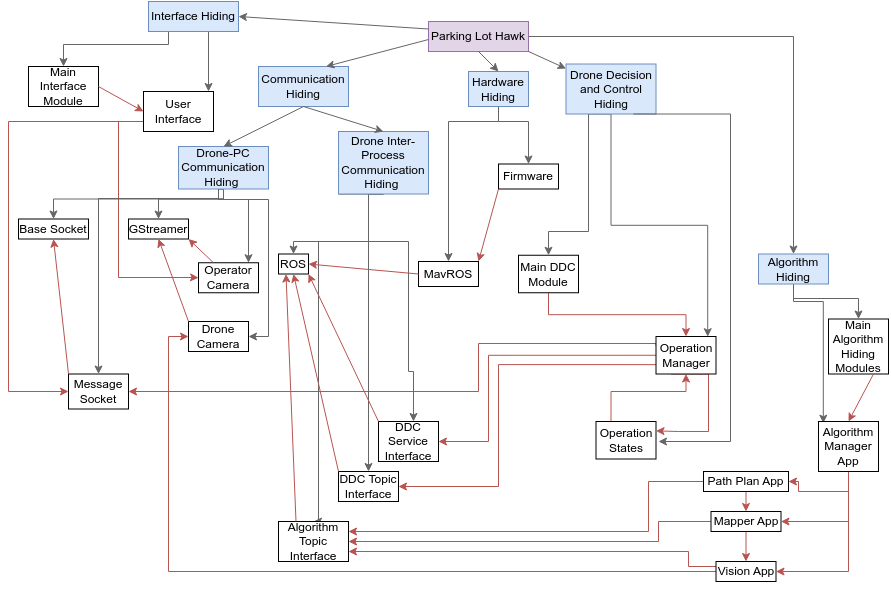
\includegraphics[width=1\textwidth]{UsesHierarchy.png}
\caption{Use hierarchy among modules}
\label{FigUH}
\end{figure}

%\section*{References}

\bibliographystyle {plainnat}
\bibliography{../../../refs/References}

\end{document}